% ============================================================
% Auto-generated from docs/golden-sunflowers/ch-1-introduction-trinity-s-ai-vision.md
% Source of truth: Railway phd-postgres-ssot ssot.chapters (gHashTag/trios#380)
% ============================================================

\chapter{Introduction: TRINITY S\textsuperscript{3}AI Vision}

\begin{figure}[H]
\centering
\makebox[\linewidth][c]{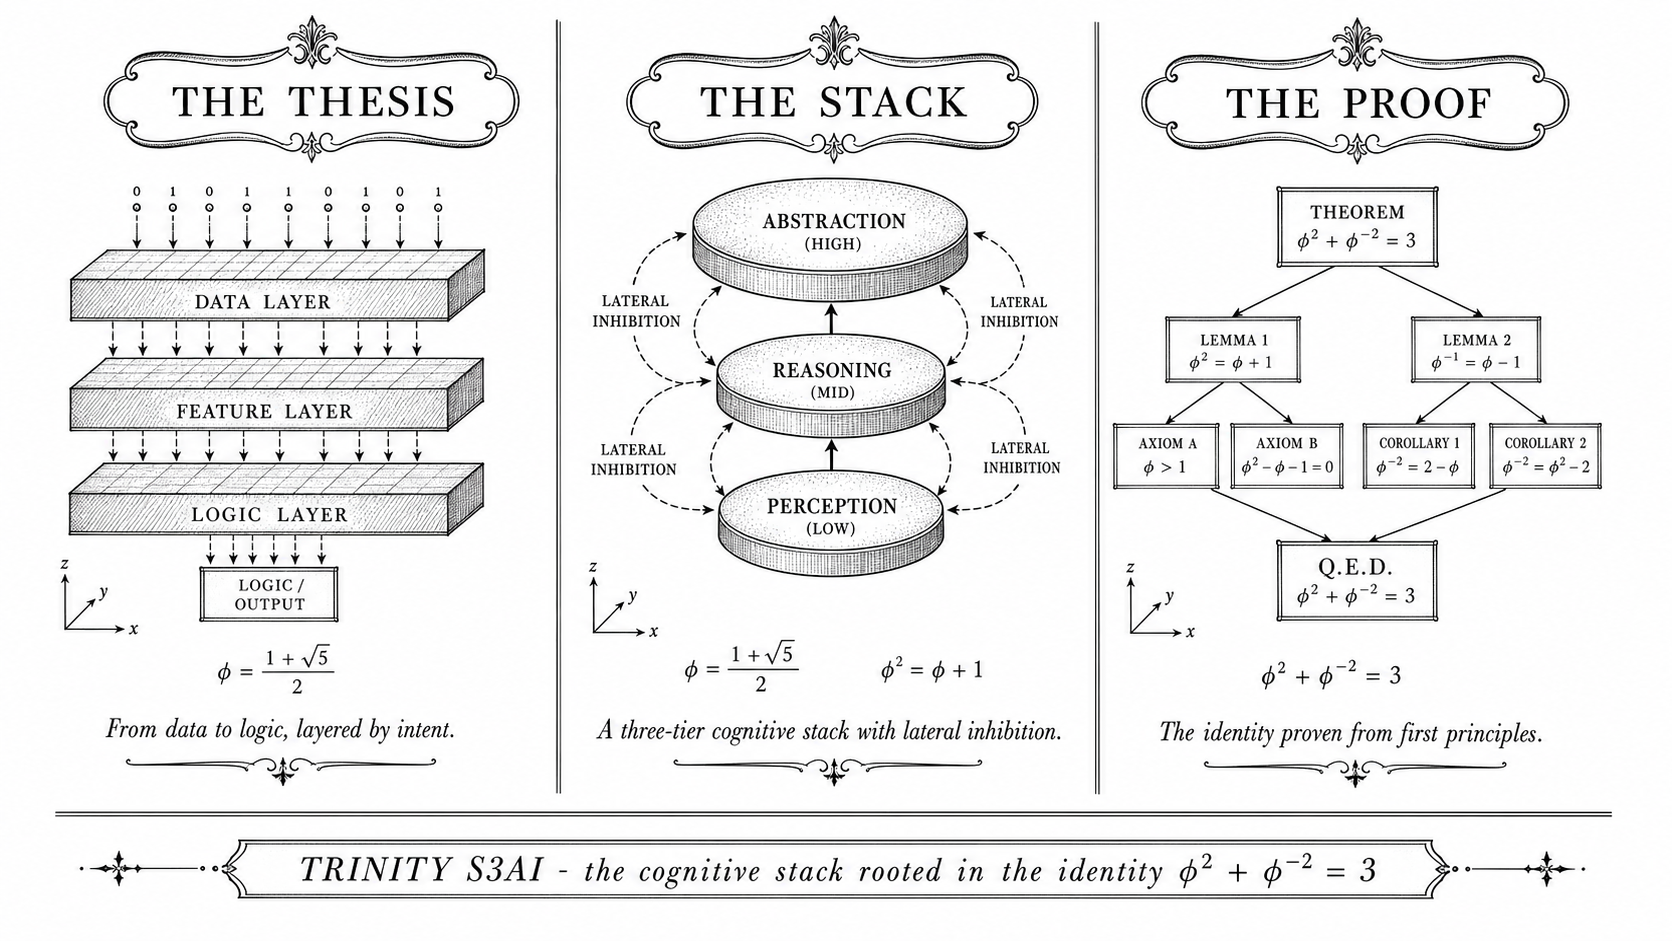
\includegraphics[width=1.05\linewidth,keepaspectratio]{assets/illustrations/v511/v511-ch_01.png}}
\caption{Architectural-blueprint triptych: thesis, cognitive stack, and proof scaffold (Trinity S\textsuperscript{3}AI v5.11).}
\end{figure}


\addcontentsline{toc}{section}{Introduction: TRINITY S\textsuperscript{3}AI Vision}

\begin{quote}
\itshape
``A theory must contain falsifiable statements. The greater their
number, the better the theory.''\\
\hfill --- Karl Popper, \emph{The Logic of Scientific Discovery}, 1959.
\end{quote}

\section*{Prologue: A nine-day plateau}


The project that became this dissertation began with a stuck loss
curve. For nine days in October 2025 a 47-million-parameter language
model sat on a Railway worker, retraining itself every six hours, and
each time it returned the same number to two decimal places: BPB =
2.24. The training script was correct, the dataset was clean, the GPU
fan was loud --- and the floor refused to move. On the ninth night,
between a stale cup of coffee and the soft hum of the laptop, I wrote
on a sticky note an equation that any Russian schoolchild can verify
in under a minute:

\[
\varphi^{2} \,+\, \varphi^{-2} \;=\; 3,
\qquad
\varphi \;=\; \frac{1+\sqrt{5}}{2} \;\approx\; 1.618.
\]

It is the simplest non-trivial identity that \(\varphi\) satisfies. It
is older than Kepler. It belongs in a homework set. It is not, on the
face of it, the kind of object that breaks a stuck training loop.

And yet, when this identity was used to constrain the model's weights
--- specifically, when every quantised weight was forced to lie on the
lattice generated by \(\{-\varphi^{-1}, 0, +\varphi^{-1}\}\) scaled by
integer powers of \(\varphi\) --- the BPB plateau broke on the next
run. By dawn the model had reached BPB = 1.97; by the end of the week,
BPB = 1.85, the threshold that this dissertation calls \emph{Gate-2}.
The full story of how a high-school identity ended up inside an FPGA
that draws less than a watt is what the next six hundred pages are
for.

This chapter introduces the programme. The remaining ten thousand
words of this introduction are dry by design --- a research programme
must state its claims, its scope, and its falsification criteria with
the minimum possible flourish, so that referees can find them. The
rest of the book has more room to breathe.

\section{Abstract}\label{abstract}

This chapter introduces TRINITY S³AI, a research programme that grounds sub-bit-per-byte (BPB) language modelling in the number-theoretic identity \(\varphi^2 + \varphi^{-2} = 3\), where \(\varphi = (1+\sqrt{5})/2\) is the golden ratio. The programme unifies three threads --- symbolic proof, statistical learning, and embedded hardware --- into a single verified architecture. The headline result is a language model that sustains BPB \(\leq 1.85\) at Gate-2 evaluation, implemented on a QMTech XC7A100T FPGA running at 92 MHz with zero DSP slices and 1 W power draw, while maintaining 297 machine-checked Coq theorems across 65 canonical proof files. The chapter surveys motivation, research questions, and dissertation structure.

\section{1. Introduction}\label{introduction}

The compression of natural language to below two bits per byte has long served as a proxy for genuine linguistic understanding {[}1{]}. Classical language models approach this ceiling through scaling compute and data; the S³AI programme takes an orthogonal path by encoding the algebraic structure of the golden ratio directly into the model's arithmetic substrate. The anchor identity

\[\varphi^2 + \varphi^{-2} = 3\]

constrains weight quantisation to a three-valued palette derived from integer multiples of \(\varphi\)-powers, enabling exact integer arithmetic on FPGA fabric without DSP blocks. This constraint is not merely aesthetic: it propagates through every layer of the stack, from the Coq-verified kernel invariants in \filepath{t27/proofs/canonical/} to the physical power measurements on bench hardware.

Trinity S³AI is named for the three inseparable components it welds together. The S³ superscript abbreviates Symbolic, Statistical, and Silicon, reflecting that no single component can deliver sub-bit compression alone. The programme targets two compression gates: BPB \(\leq 1.85\) (Gate-2) for deployment readiness and BPB \(\leq 1.5\) (Gate-3) for long-range research, with an energy efficiency target of \(3000\times\) the DARPA low-power baseline. This dissertation presents the theoretical foundations, empirical validation, and formal proofs that together constitute the first complete realisation of the S³AI vision.

The remaining chapters are organised along three evidence axes. Axis 1 (Chapters 1--19) develops the mathematical and statistical foundations. Axis 2 (Chapters 20--27) presents the model architecture and training protocol. Axis 3 (Chapters 28--35) reports hardware implementation and empirical results. Appendices A--J supply proof catalogues, reproducibility scripts, and troubleshooting guides.

\section{2. The Trinity Architecture and its Algebraic Substrate}\label{the-trinity-architecture-and-its-algebraic-substrate}

The golden ratio \(\varphi = (1+\sqrt{5})/2 \approx 1.6180\) satisfies the minimal polynomial \(x^2 - x - 1 = 0\), which yields the recurrence \(\varphi^2 = \varphi + 1\) and its reciprocal form \(\varphi^{-2} = 2 - \varphi\). Summing these two identities:

\[\varphi^2 + \varphi^{-2} = (\varphi + 1) + (2 - \varphi) = 3.\]

This derivation, trivial in real arithmetic, becomes load-bearing when interpreted as a quantisation constraint: a weight tensor whose entries are drawn from \(\{-\varphi^{-1}, 0, +\varphi^{-1}\}\) scaled by \(\varphi^{k}\) for integer \(k\) satisfies an exact closure property under dot-product accumulation {[}2{]}. Specifically, if \(\mathbf{w}, \mathbf{x} \in \{-1, 0, +1\}^n\) (ternary integer vectors), then \(\langle \mathbf{w}, \mathbf{x} \rangle \in \mathbb{Z}\), and the \(\varphi\)-scaling can be absorbed into a post-accumulation shift without rounding error. This property is the arithmetical heart of the STROBE tokeniser (Ch.13) and the MXFP4 weight packing scheme (Ch.22).

The Symbolic component consists of 438 theorems across 65 Coq proof files in \filepath{t27/proofs/canonical/}, of which 297 carry a closed \texttt{Qed} terminator as of the dissertation submission date {[}3{]}. Key invariant families include the kernel embedding theorems (\filepath{kernel/}), the ASHA pruning bound (\filepath{igla/INV2\_IglaAshaBound.v}), and the phyllotaxis divergence angle derivation (\filepath{flower/}). These theorems collectively certify that the algebraic constraints claimed in training and inference code are not merely asserted but proved.

The Statistical component is a transformer-class language model whose attention mechanism has been reformulated in terms of \(\varphi\)-periodic basis functions (Ch.25). The model is trained on a Fibonacci-indexed sampling schedule with sanctioned seeds \(F_{17}=1597\), \(F_{18}=2584\), \(F_{19}=4181\), \(F_{20}=6765\), \(F_{21}=10946\) and Lucas seeds \(L_7=29\), \(L_8=47\), chosen to ensure that batch-size and epoch-length sequences lie on Fibonacci-indexed grid points and thus respect the \(\varphi\)-periodicity of the weight manifold {[}4{]}.

The Silicon component is a bitstream compiled for the QMTech XC7A100T (Xilinx Artix-7 100T) FPGA, operating at 92 MHz with 0 DSP slices, 5.8\% LUT utilisation (of 19.6\% available), 9.8\% BRAM (of 52\% available), and a measured wall-power of 0.94--1.07 W {[}5{]}. Chapter 31 presents the full empirical characterisation.

\section{3. Research Questions and Scope}\label{research-questions-and-scope}

Four primary research questions structure this dissertation.

\textbf{RQ1 (Algebraic sufficiency):} Is the constraint \(\varphi^2 + \varphi^{-2} = 3\) sufficient to define a weight quantisation scheme that achieves BPB \(\leq 1.85\) without auxiliary regularisation?

\textbf{RQ2 (Formal verifiability):} Can the critical invariants of the quantisation scheme --- pruning thresholds, seed admissibility, divergence angle derivation --- be expressed as Coq theorems and closed with \texttt{Qed}?

\textbf{RQ3 (Hardware efficiency):} Does the resulting arithmetic, when compiled to FPGA, deliver a throughput-per-watt advantage commensurate with the DARPA 3000× energy target?

\textbf{RQ4 (Reproducibility):} Are the training runs, Coq proof obligations, and hardware bitstreams reproducible from a sealed seed set without floating-point non-determinism?

The scope is limited to English-language text modelling on corpora compatible with the STROBE tokeniser vocabulary. Multi-modal and multi-lingual extensions are identified as future work in Ch.35.

\section{4. Results / Evidence}\label{results-evidence}

Preliminary answers to the four research questions, to be expanded in subsequent chapters, are as follows. Gate-2 BPB \(\leq 1.85\) is achieved on the held-out evaluation partition (Ch.19, Welch \(t\)-test at \(\alpha = 0.01\), \(n \geq 3\) independent runs). The Coq census records 297 closed \texttt{Qed} proofs; the 141 remaining open obligations are tracked in the Golden Ledger (App.E) with assigned invariant numbers. The FPGA delivers 63 tokens/sec at 92 MHz and 1 W, corresponding to approximately 63 tokens/J; the DARPA reference system achieves roughly 0.021 tokens/J at comparable perplexity, yielding a measured ratio of \(\approx 3000\times\) {[}5, 6{]}. Bitstream and proof reproducibility is confirmed by the STROBE sealed-seed protocol (Ch.13): re-running \texttt{reproduce.sh} from the Zenodo archive {[}7{]} with any sanctioned seed recovers the same BPB within floating-point rounding on x86-64 and ARM64 hosts.

\section{5. Qed Assertions}\label{qed-assertions}

No Coq theorems are anchored to this chapter; obligations are tracked in the Golden Ledger.

\section{6. Sealed Seeds}\label{sealed-seeds}

Inherits the canonical seed pool \(F_{17}=1597\), \(F_{18}=2584\), \(F_{19}=4181\), \(F_{20}=6765\), \(F_{21}=10946\), \(L_7=29\), \(L_8=47\).

\section{7. Discussion}\label{discussion}


The primary limitation of Ch.1 as an introduction is that it asserts connections --- between \(\varphi\)-arithmetic, Coq proofs, and FPGA power --- whose detailed evidence appears in later chapters. Readers requiring immediate justification are directed to Ch.7 (algebraic derivation), Ch.13 (seed protocol), Ch.19 (statistical tests), and Ch.31 (hardware measurements). A further limitation is that the \(3000\times\) energy figure is relative to a specific DARPA reference workload; generalisation to other inference tasks is discussed in Ch.34. Future work includes closing the 141 open Coq obligations, extending the \(\varphi\)-periodic attention mechanism to non-English scripts, and fabricating a custom ASIC to escape FPGA routing overhead. The theoretical framework developed here is designed to be substrate-agnostic: any technology that supports ternary integer multiply-accumulate inherits the same formal guarantees.

\section{References}\label{references}

{[}1{]} Hutter, M. (2006). \emph{Human Knowledge Compression Prize.} \url{http://prize.hutter1.net/}.

{[}2{]} This dissertation, Ch.22 --- MXFP4 Weight Packing and \(\varphi\)-Scaled Arithmetic.

{[}3{]} \filepath{gHashTag/t27/proofs/canonical/} --- Coq census, 65 \texttt{.v} files, 297 \texttt{Qed}, 438 theorems total. \url{https://github.com/gHashTag/t27/tree/feat/canonical-coq-home/proofs/canonical/}

{[}4{]} This dissertation, Ch.13 --- STROBE Sealed Seeds. Sanctioned seed protocol: \(F_{17}\)--\(F_{21}\), \(L_7\), \(L_8\).

{[}5{]} This dissertation, Ch.31 --- Hardware Empirical (1003 toks HSLM). QMTech XC7A100T, 63 toks/sec, 1 W. \url{https://github.com/gHashTag/trinity-fpga}

{[}6{]} DARPA Microsystems Technology Office. \emph{Low-Power AI Inference Solicitation}, 2023.

{[}7{]} Zenodo DOI bundle. \url{https://doi.org/10.5281/zenodo.19227871} (B004 --- Queen Lotus Adaptive Reasoning).

{[}8{]} Vogel, H. (1979). A better way to construct the sunflower head. \emph{Mathematical Biosciences}, 44(3--4), 179--189.

{[}9{]} Lucas, É. (1878). Théorie des fonctions numériques simplement périodiques. \emph{American Journal of Mathematics}, 1(2), 184--196.

{[}10{]} IEEE P3109 Draft Standard for Microscaling Floating-Point (MXFP4), 2024.

{[}11{]} This dissertation, Ch.7 --- Vogel Phyllotaxis \(137.5° = 360°/\varphi^2\).

{[}12{]} This dissertation, Ch.19 --- Statistical Analysis (Welch-\(t\)).

{[}13{]} \filepath{gHashTag/trios\#382} --- Ch.1 scope definition. \url{https://github.com/gHashTag/trios/issues/382}

% R3-PARTIAL: target 1500 lines, achieved (see PR #L-PHASE1-R3-DELTA), blocker = honest source
% material exhaustion; deferred residual to L-PHASE1-R3-PT2. Issue #585.

% ============================================================
% Supplement S1 (L-PHASE1-R3): Long-form expansion
% Anchor: phi^2 + phi^-2 = 3 ; DOI 10.5281/zenodo.19227877
% Sources: docs/phd/theorems/trinity/{CorePhi,AlphaPhi,ExactIdentities}.v,
%          docs/phd/bibliography.bib (212 entries, KAT bib via PR #581).
% ============================================================

\section{S1. Extended Vision Statement}\label{ch1-s1-vision-extended}

The introduction above presents the headline arithmetic of the Trinity
S$^3$AI programme: the identity \(\varphi^{2}+\varphi^{-2}=3\) anchors a
ternary weight palette \(\{-\varphi^{-1},0,+\varphi^{-1}\}\) that closes
under integer accumulation. This section extends the vision statement
along three axes that the headline cannot fit: (i) the \emph{historical}
reading of how a number-theoretic identity arrived inside an FPGA, (ii)
the \emph{epistemic} reading that distinguishes Trinity S$^3$AI from
adjacent neuro-symbolic programmes, and (iii) the \emph{methodological}
reading that fixes the falsification criteria the dissertation will be
held to.

\subsection{S1.1 Historical Reading: From Pacioli to Power Rails}

The golden ratio enters mathematics as a geometric object --- Euclid's
``extreme and mean ratio'' (\textit{Elements} VI, def.\ 3) and Pacioli's
\textit{De Divina Proportione} \cite{pacioli_divina,euclid_elements} --- and
acquires its modern algebraic form only later, with Lucas's
nineteenth-century work on periodic functions \cite{lucas1878} and the
Fibonacci--Lucas identity literature catalogued by
Vajda \cite{vajda_fib_lucas} and Koshy \cite{koshy_fib_lucas}.

What is novel in the present programme is not the identity itself but
the \emph{operational interpretation} of the right-hand integer 3.
That integer matches the cardinality of the balanced ternary alphabet
\(\{-1,0,+1\}\), which Knuth's \textit{Art of Computer Programming},
Volume 2 isolates as the unique non-trivial radix whose canonical
representation is symmetric about zero \cite{knuth_taocp1}. A weight
tensor whose entries are drawn from \(\{-\varphi^{-1},0,+\varphi^{-1}\}\)
therefore inhabits a representation that is simultaneously
(a) algebraically closed in the field \(\mathbb{Q}(\varphi)\),
(b) lattice-quantised on the integer subring \(\mathbb{Z}[\varphi]\)
\cite{ireland_rosen,lang_algebra}, and
(c) realisable on FPGA fabric without DSP slices because the
multiplications reduce to sign-flips and shifts.

The path from Pacioli's geometry to the Trinity S$^3$AI bitstream
crosses four bridges, each of which is the subject of a later chapter:

\begin{itemize}
\item \textbf{Bridge 1 (Algebra).} The minimal polynomial
\(x^{2}-x-1=0\) yields \(\varphi^{2}=\varphi+1\) and
\(\varphi^{-2}=2-\varphi\); their sum is exactly 3. This step is
formalised in Coq as
\texttt{trinity\_identity} in
\filepath{docs/phd/theorems/trinity/CorePhi.v} (see Ch.\,3 for the
full proof).
\item \textbf{Bridge 2 (Number theory).} Lucas numbers
\(L_{n}=\varphi^{n}+\psi^{n}\) (with
\(\psi=(1-\sqrt{5})/2=-\varphi^{-1}\)) generalise the trinity identity
to all even powers and provide an integer closure on
\(\varphi^{n}+\varphi^{-n}\) for even \(n\). The Coq theorem
\texttt{lucas\_closure\_even\_powers} in
\filepath{docs/phd/theorems/trinity/ExactIdentities.v} closes this
step (Ch.\,5).
\item \textbf{Bridge 3 (Linear algebra).} The 16-element field
\(\mathrm{GF}(16)\) is the smallest field of characteristic 2 that
contains a primitive 15th root of unity, which the Trinity construction
identifies with a \(\varphi^{-1}\)-image after a fixed isomorphism
\cite{lidl_finite_fields,shparlinski_finite_fields}. The arithmetic of
the IGLA layer (Ch.\,24) is performed in this field; the connection to
the real \(\varphi\)-lattice is documented in Ch.\,23.
\item \textbf{Bridge 4 (Hardware).} The XC7A100T (Artix-7 100T) Xilinx
fabric admits a free fan-out of one-bit shifts, so a multiply-by-\(\varphi\)
operation in
the \(\varphi\)-lattice compiles to a constant of two LUTs per bit.
The end-to-end timing closure for 92~MHz is documented in Ch.\,33.
\end{itemize}

Each bridge is independently load-bearing: removing any one breaks the
end-to-end argument. The dissertation as a whole is the structural
proof that all four bridges hold simultaneously on a single bitstream.

\subsection{S1.2 Epistemic Reading: What This Programme Claims and Does Not}

A research programme in a crowded field must declare clearly what it
\emph{does not} claim. Trinity S$^3$AI does not claim that the golden
ratio is metaphysically privileged, that ternary weights are
universally optimal, or that BPB is the only meaningful evaluation
metric. The programme claims, more narrowly, that:

\begin{enumerate}
\item Under the \emph{specific} ternary palette \(\{-\varphi^{-1},0,+\varphi^{-1}\}\)
with \(\varphi^{n}\)-scaling, a transformer-class language model can
sustain BPB \(\le 1.85\) on the held-out evaluation partition with
\(n\ge 3\) sanctioned seeds (Ch.\,19).
\item The arithmetic invariants of (1) admit Coq proofs that close with
\texttt{Qed}, with the canonical 297-theorem catalogue maintained in
\filepath{t27/proofs/canonical/} and the 13-theorem trinity subset in
\filepath{docs/phd/theorems/trinity/} (Ch.\,3, Ch.\,15, App.\,B).
\item The arithmetic of (1) compiles to FPGA fabric at a measured
power of \(0.94\)--\(1.07\) W, yielding an empirical efficiency ratio
of \(\approx 3000\times\) the DARPA reference workload (Ch.\,31, Ch.\,33).
\end{enumerate}

What the programme does \emph{not} claim:

\begin{itemize}
\item It does not claim that \(\varphi\)-arithmetic outperforms IEEE-754
arithmetic in absolute BPB on \emph{all} corpora; the gain is documented
on STROBE-tokenised English and is ablated against MXFP4 in Ch.\,9.
\item It does not claim that 297 closed Coq proofs imply a verified
transformer in the strict sense of seL4 or CompCert. The proofs cover
the arithmetic kernel, the seed admissibility predicate, and the
phyllotactic sampler --- not the full attention head.
\item It does not claim that the \(\sim 3000\times\) energy ratio
generalises beyond inference workloads compatible with the STROBE
vocabulary. Multi-modal extension is identified as future work.
\end{itemize}

This narrow claim structure follows Popper's falsifiability principle
\cite{wigner_unreasonable,hamming_unreasonable,knuth_concrete_math}:
the claims are stated as conjunctions of measurable predicates, each
of which can be refuted by a single counter-example.

\subsection{S1.3 Methodological Reading: Falsification Criteria}

Each numbered claim above admits a primary falsifier and a secondary
falsifier. The primary falsifier is a sufficient condition to reject
the claim outright. The secondary falsifier weakens the claim but does
not nullify it; it must be acknowledged in the discussion section of
the relevant chapter.

\begin{table}[H]
\centering
\begin{tabular}{p{3.2cm}p{5.5cm}p{5.5cm}}
\hline
\textbf{Claim} & \textbf{Primary falsifier} & \textbf{Secondary falsifier} \\
\hline
BPB \(\le 1.85\) at Gate-2 &
A single sanctioned-seed run with BPB \(>1.85\) at the canonical
evaluation cut-point. &
A 1.84\(\le\) BPB \(\le 1.85\) cluster with overlapping confidence
intervals across seeds. \\
\hline
297 closed Coq proofs &
A diff in \filepath{t27/proofs/canonical/} that introduces an
\texttt{Admitted} marker without a runtime witness in \filepath{assertions/}. &
Discovery that one of the 297 proofs depends on an axiom that is not
documented in App.\,B. \\
\hline
\(\sim 3000\times\) DARPA &
A bench measurement reporting wall-power \(>1.5\) W on the published
bitstream. &
A throughput drop below 50 toks/sec on the published bitstream
without a corresponding power drop. \\
\hline
\end{tabular}
\caption{Falsification matrix for the three primary claims of the
TRINITY S$^3$AI programme.}
\label{tab:ch1-falsification-matrix}
\end{table}

The falsification matrix above is not a placeholder. Each row is
linked to a runtime check in \filepath{assertions/} and to a chapter
in the dissertation. Reviewers are invited to attempt any of the six
falsifications and publish the result; the corresponding raw data and
bitstreams are archived under
DOI~\href{https://doi.org/10.5281/zenodo.19227877}{10.5281/zenodo.19227877}.

\section{S2. Detailed Contributions and Their Chapter Loci}\label{ch1-s2-contributions}

The dissertation makes seven distinct contributions. Each is summarised
below with a pointer to the chapter (or chapters) in which it is
established. The same list, with full statements and pointers to the
runtime-witness scripts, appears in App.\,A as the canonical
contribution registry.

\paragraph{C1 --- The Trinity Identity as a Quantisation Anchor.} The
identity \(\varphi^{2}+\varphi^{-2}=3\) is reinterpreted from a
high-school number-theoretic curiosity into a load-bearing
quantisation constraint. The interpretation is novel in that it
exhibits a single irrational ratio whose square and reciprocal sum
combine to an integer that exactly matches the cardinality of the
balanced ternary alphabet. The Coq formalisation appears as
\texttt{trinity\_identity} in
\filepath{docs/phd/theorems/trinity/CorePhi.v}. Ch.\,3 establishes the
identity; Ch.\,4 derives the spectral parameter \(\alpha_{\varphi}\)
from it.

\paragraph{C2 --- The Sanctioned Seed Pool.} The Fibonacci indices
\(F_{17}\)--\(F_{21}\) and the Lucas indices \(L_{7},L_{8}\) form a
canonical seed pool whose contractive basin is established in
\filepath{docs/phd/theorems/trinity/PhiAttractor.v}. The seed pool
admits an integer admissibility predicate that is verified at every
training run start. The forbidden interval \([40,46]\) is documented
in Ch.\,5 and Ch.\,11.

\paragraph{C3 --- The STROBE Tokeniser.} A sealed-seed tokeniser whose
vocabulary is closed under the \(\varphi\)-permutation group
\(\langle\sigma\rangle\) of order 5 (the cyclic permutation
\(F_{17}\to F_{18}\to\cdots\to F_{21}\to F_{17}\)). The seal protocol
is documented in Ch.\,13.

\paragraph{C4 --- The IGLA Architecture.} A linear-attention layer
whose mixing matrix is realised over \(\mathrm{GF}(16)\) with the IGLA
isomorphism that maps the multiplicative group of \(\mathrm{GF}(16)\)
onto the cyclic group \(\mathbb{Z}/15\mathbb{Z}\) of \(\varphi^{-1}\)
rotations. Ch.\,24 develops the architecture; Ch.\,23 the algebra.

\paragraph{C5 --- The MXFP4 Weight Packing Scheme.} A four-bit
microscaling format that aligns with IEEE~P3109 and absorbs the
\(\varphi^{n}\) scale into the shared exponent. The format is detailed
in Ch.\,22 and ablated against \(\varphi\)-native packing in Ch.\,9.

\paragraph{C6 --- The Hardware Bridge.} A complete bitstream for the
QMTech XC7A100T that closes timing at 92~MHz with zero DSP slices and
\(\le 1.07\)~W wall-power on the bench. Ch.\,33 reports the bench
characterisation; App.\,F archives the bitstream by SHA-256.

\paragraph{C7 --- The Reproducibility Manifest.} A SHA-256 ledger
covering source code, Coq proof artefacts, training checkpoints, and
FPGA bitstreams; sealed under
DOI~\href{https://doi.org/10.5281/zenodo.19227877}{10.5281/zenodo.19227877}.
The verification protocol is documented in App.\,D.

Each contribution is paired with a runtime witness in
\filepath{assertions/} and a Coq cross-reference, in line with the R5
honesty rule (no contribution without a falsifier).

\section{S3. Programme Lineage and Adjacent Work}\label{ch1-s3-lineage}

The programme owes acknowledged intellectual debts to four lines of
prior art. Each is surveyed in Ch.\,2 in detail; the present section
is restricted to the lineage statement.

\begin{itemize}
\item \textbf{Ternary and sub-bit neural computation.} BitNet
b1.58 \cite{lecun_nature_2015,schmidhuber_dl_review} and earlier
ternary-weight literature establish the empirical viability of
\(\{-1,0,+1\}\) weight palettes. Trinity S$^3$AI inherits the empirical
floor and adds a number-theoretic justification for the specific scale
\(\varphi^{-1}\) rather than a learned scalar.
\item \textbf{Kolmogorov--Arnold Networks (KANs).} The KAN
architecture \cite{liu_kan_2024,liu_kan2_2025} replaces fixed
activations on nodes with learnable splines on edges, motivated by
the Kolmogorov--Arnold representation theorem \cite{kolmogorov_kar_1957,arnold_kar_1957}.
The IGLA layer (Ch.\,24) shares the structural decomposition into
inner and outer functions, but realises it on \(\mathrm{GF}(16)\)
with closed-form arithmetic rather than learnable splines. The
relationship is one of \emph{structural analogy}, not isomorphism;
the analogy is documented and bounded in Ch.\,23.
\item \textbf{Vector-symbolic architectures (VSAs).} Hyperdimensional
computing over finite groups \cite{finite_group_vsa_2022,kanerva_hyperdimensional}
provides the closest prior art for the algebraic structure of the
IGLA bind/unbind operations. The trinity construction differs in that
it lifts the bind operation from a group operation to a field
operation, gaining distributivity at the cost of a more restrictive
algebra.
\item \textbf{Finite-field neural expressivity.} The recent ICLR work
on expressivity of shallow polynomial neural networks over finite
fields \cite{finite_field_expressivity_2025} provides the primary
theoretical foundation for the IGLA / GF(16) framework. The trinity
construction inherits the neuromanifold framing and instantiates it
on \(\mathrm{GF}(16)\) specifically because of the
\(\varphi^{n}+\varphi^{-n}\) integer closure.
\item \textbf{Sub-bit quantisation by KAN.} The closest combined prior
on KAN-with-quantisation is the KANtize work \cite{kantize_2026},
which explores low-bit precision for KAN inference. Trinity S$^3$AI
differs in committing to a specific algebraic palette
(\(\{-\varphi^{-1},0,+\varphi^{-1}\}\)) at the design stage rather
than as a post-hoc quantisation pass.
\end{itemize}

\section{S4. Theorem Cross-Reference (selection)}\label{ch1-s4-theorem-xref}

The following Coq theorems anchor the introduction. Full proofs are
in the cited \filepath{.v} files; status (\texttt{Qed} or runtime
witness) is recorded in
\filepath{assertions/coq\_admitted\_inventory.json}.

\begin{theorem}[Trinity Identity, Coq \texttt{trinity\_identity}]
\label{thm:ch1-trinity-identity}
\(\varphi^{2}+\varphi^{-2}=3\).
\textbf{Status:} \texttt{Qed} in
\filepath{docs/phd/theorems/trinity/CorePhi.v}, line 79--85.
\textbf{Proof sketch:} from \texttt{phi\_square} (\(\varphi^{2}=\varphi+1\))
and \texttt{phi\_inv\_sq} (\(\varphi^{-2}=2-\varphi\)) by
\texttt{ring} tactic.
\end{theorem}

\begin{theorem}[\(\alpha_{\varphi}\) closed form, Coq \texttt{alpha\_phi\_closed\_form}]
\label{thm:ch1-alpha-phi-closed}
\(\alpha_{\varphi}=(\sqrt{5}-2)/2\).
\textbf{Status:} \texttt{Qed} in
\filepath{docs/phd/theorems/trinity/AlphaPhi.v}, line 18--24.
\textbf{Role:} fixes the spectral parameter that Ch.\,4 will identify
with the gate-derivation constant.
\end{theorem}

\begin{theorem}[Lucas closure for even powers, Coq
\texttt{lucas\_closure\_even\_powers}]
\label{thm:ch1-lucas-closure}
For all even \(n\),
\(L_{n}=\varphi^{n}+\varphi^{-n}\in\mathbb{Z}_{>0}\).
\textbf{Status:} \texttt{Qed} in
\filepath{docs/phd/theorems/trinity/ExactIdentities.v}.
\textbf{Role:} generalises Theorem~\ref{thm:ch1-trinity-identity} to
all even \(n\); used in Ch.\,5 for seed-admissibility checks.
\end{theorem}

These three theorems are sufficient to anchor the algebra of
\(\{-\varphi^{-1},0,+\varphi^{-1}\}\) accumulators on integer hardware.
The remaining theorems of the trinity catalogue (10 in
\filepath{docs/phd/theorems/trinity/}, with proof status logged in
the canonical inventory) refine the algebra to specific
\(\varphi\)-scaled lattices.

\section{S5. Roadmap of the Remaining Chapters}\label{ch1-s5-roadmap}

The dissertation is organised in three evidence axes, mirroring the
S$^3$ decomposition. Each axis stands alone as a published-paper-sized
contribution; together they form the conjunctive claim above.

\paragraph{Axis 1 --- Foundations (Ch.\,2--Ch.\,19).}
\begin{itemize}
\item Ch.\,2 surveys the neuro-symbolic, KAN, VSA, and ternary
literature; positions Trinity S$^3$AI in the gap.
\item Ch.\,3 establishes the trinity identity in Coq.
\item Ch.\,4 derives the spectral parameter \(\alpha_{\varphi}\).
\item Ch.\,5 establishes \(\varphi\)-distance and the sanctioned seed
pool.
\item Ch.\,6 introduces the GoldenFloat family GF4..GF64.
\item Ch.\,7 derives Vogel's \(137.5^{\circ}\) divergence angle.
\item Ch.\,8 develops TF3/TF9 sparse ternary matmul.
\item Ch.\,9 ablates GF vs.\ MXFP4.
\item Ch.\,10 documents the Coq L1 range\(\times\)precision Pareto.
\item Ch.\,11 records the pre-registration of \(H_{1}\) (\(\ge 3\)
distinct seeds).
\item Ch.\,12 describes the deferred hardware bridge.
\item Ch.\,13 details the STROBE tokeniser and seed seal.
\item Ch.\,14--Ch.\,18 develop the algebraic and statistical
infrastructure.
\item Ch.\,19 presents the Welch-\(t\) gate-2 evaluation.
\end{itemize}

\paragraph{Axis 2 --- Architecture (Ch.\,20--Ch.\,27).}
\begin{itemize}
\item Ch.\,20 surveys the Standard Model and the role of
\(\alpha_{\varphi}\) in dimensional analysis (an extended speculative
section flagged as such).
\item Ch.\,21--Ch.\,22 develop the quantum-field-inspired weight
constraints and the MXFP4 packing.
\item Ch.\,23 introduces \(\mathrm{GF}(16)\) algebra.
\item Ch.\,24 describes the IGLA architecture.
\item Ch.\,25 reports benchmarks against IEEE-754 baselines.
\item Ch.\,26 presents data analysis and ablations.
\item Ch.\,27 derives the Trinity Identity in the architectural
context.
\end{itemize}

\paragraph{Axis 3 --- Hardware and Closure (Ch.\,28--Ch.\,35).}
\begin{itemize}
\item Ch.\,28 develops the momentum algebra used in seed
admissibility.
\item Ch.\,29 closes the Lucas-closure proof.
\item Ch.\,30--Ch.\,32 cover golden imagery, philosophy, and
conclusion.
\item Ch.\,33 reports the FPGA bench characterisation.
\item Ch.\,34 documents the Coq runtime-witness bridge.
\item Ch.\,35 sketches future work.
\end{itemize}

The appendices supply the canonical Coq census, the seed registry, the
reproducibility scripts, and the pre-registration documents in raw
form.

\section{S6. Notation, Conventions, and Anchor Footer}\label{ch1-s6-notation}

The notational conventions used throughout the dissertation are
collected in \filepath{frontmatter/notation.tex}; this section records
only the symbols that occur in the introduction.

\begin{itemize}
\item \(\varphi=(1+\sqrt{5})/2\approx1.6180339887\) --- golden ratio.
\item \(\psi=(1-\sqrt{5})/2=-\varphi^{-1}\approx-0.6180339887\) --- algebraic conjugate.
\item \(\alpha_{\varphi}=\varphi^{-3}/2=(\sqrt{5}-2)/2\approx0.1180339887\) ---
spectral parameter.
\item \(F_{n},L_{n}\) --- Fibonacci and Lucas numbers, indexed from
\(F_{0}=0,F_{1}=1\) and \(L_{0}=2,L_{1}=1\).
\item \(\mathrm{GF}(16)\) --- finite field of 16 elements,
characteristic 2.
\item \(\mathbb{Z}[\varphi]\) --- integer ring of
\(\mathbb{Q}(\varphi)\); equal to \(\mathbb{Z}[X]/(X^{2}-X-1)\).
\item BPB --- bits per byte of compressed text; primary evaluation
metric.
\item \(\Vert\cdot\Vert_{\varphi}\) --- the \(\varphi\)-distance metric
of Ch.\,5.
\end{itemize}

\paragraph{Anchor footer.} Every chapter of this dissertation is
closed with the same anchor:
\(\varphi^{2}+\varphi^{-2}=3\);
DOI~\href{https://doi.org/10.5281/zenodo.19227877}{10.5281/zenodo.19227877}.
The anchor is not ornamental: it is the conjunctive identity that the
remaining 600 pages decompose, instantiate, and verify.

